\documentclass{article}

% if you need to pass options to natbib, use, e.g.:
% \PassOptionsToPackage{numbers, compress}{natbib}
% before loading nips_2017
%
% to avoid loading the natbib package, add option nonatbib:
% \usepackage[nonatbib]{nips_2017}

\usepackage{graphicx}
\usepackage{nips_2017}

% to compile a camera-ready version, add the [final] option, e.g.:
% \usepackage[final]{nips_2017}

\usepackage[utf8]{inputenc} % allow utf-8 input
\usepackage[T1]{fontenc}    % use 8-bit T1 fonts
\usepackage{hyperref}       % hyperlinks
\usepackage{url}            % simple URL typesetting
\usepackage{booktabs}       % professional-quality tables
\usepackage{amsfonts}       % blackboard math symbols
\usepackage{nicefrac}       % compact symbols for 1/2, etc.
\usepackage{microtype}      % microtypography

\title{Detecting Credit Card Fraud in a Skewed Data Set Using Deep Learning}

% The \author macro works with any number of authors. There are two
% commands used to separate the names and addresses of multiple
% authors: \And and \AND.
%
% Using \And between authors leaves it to LaTeX to determine where to
% break the lines. Using \AND forces a line break at that point. So,
% if LaTeX puts 3 of 4 authors names on the first line, and the last
% on the second line, try using \AND instead of \And before the third
% author name.

\author{
  Isaac Smith \\
  Department of Computer Science\\
  South Dakota School of Mines & Technology\\
  Rapid City, SD 57110 \\
  %% examples of more authors
  %% \And
  %% Coauthor \\
  %% Affiliation \\
  %% Address \\
  %% \texttt{email} \\
  %% \AND
  %% Coauthor \\
  %% Affiliation \\
  %% Address \\
  %% \texttt{email} \\
  %% \And
  %% Coauthor \\
  %% Affiliation \\
  %% Address \\
  %% \texttt{email} \\
  %% \And
  %% Coauthor \\
  %% Affiliation \\
  %% Address \\
  %% \texttt{email} \\
}

\begin{document}
% \nipsfinalcopy is no longer used

\maketitle

\begin{abstract}
 Deep learning can be used in various financial applications, one such being
 monitoring for fraudulent credit card activity. Using a dataset of over 280,000
 credit card transaction data points, each data point can be fed into a neural network
 and train the network to differentiate the features of a fraudulent transaction vs. 
a non-fraudulent transaction. Optimizing the hyperparameters of the network can
 push the accuracy into the high 99\% range and could potentially identify all
 cases with a relatively high confidence. This confidence could then be applied
 to credit monitoring agencies to assist in protecting consumers.
\end{abstract}

\section{Introduction}

 Credit card fraud is a problem for many people across the United States,
 with 45,428 cases of credit card fraud reported to the Federal Trade Commission in 2017 [1].
 With datasets available today, neural networks can be trained to identify trends
 in fraudulent and non-fraudulent transactions.

 The output of these networks can be used to notify consumers of
 suspicious activity on their accounts and prevent further losses.


\subsection{The Dataset}


For this case study, the dataset consists of over 280,000 credit card transaction 
data points accumulated over 2 days in European countries\footnote{Dataset from
 https://www.kaggle.com/mlg-ulb/creditcardfraud/data.}. Each data point 
holds basic information about the transaction as well as obfuscated data resulting 
from a PCA transformation, which can be seen in Table~\ref{sample-points}. The data 
prefixed with a “V” is the transformed data.

\begin{table}[htb]
  \caption{Sample Transaction Data Points}
  \label{sample-points}
  \centering
  \begin{tabular}{llllllll}	
    \toprule
    Time & V1 & V2  & ... & V27 & V28 & Amount & Class \\
    \midrule
    0 & -1.359807134  & -0.072781173 &    ...    & 0.133558377 & -0.021053053 & 149.62 & 0    \\
    70071 & -0.440095203  & 1.137238976 &    ...    & 0.768290751 & 0.459623328 & 227.3 & 1    \\
    132086 & -0.361427839 & 1.133471917 &    ...    & -0.001249817 & -0.182750897 & 480.72 & 1 \\
    150426 & -0.269118964  & -0.063708356 &    ...    & 0.385434237 & 0.21311729 & 7.33 & 0    \\
    172792 & -0.533412522  & -0.189733337 &    ...    & -0.002415309 & 0.013648914 & 217 & 0    \\
    \bottomrule
  \end{tabular}
\end{table}

 One of the interesting metrics of the dataset is the ratio of fraudulent to non-fraudulent transactions. 
 With fraudulent transactions only making up 0.172\% of the 280,000+ transactions, this poses a 
 challenge for a neural network to make accurate identifications for fraudulent cases. 

\begin{figure}
  \begin{center}
    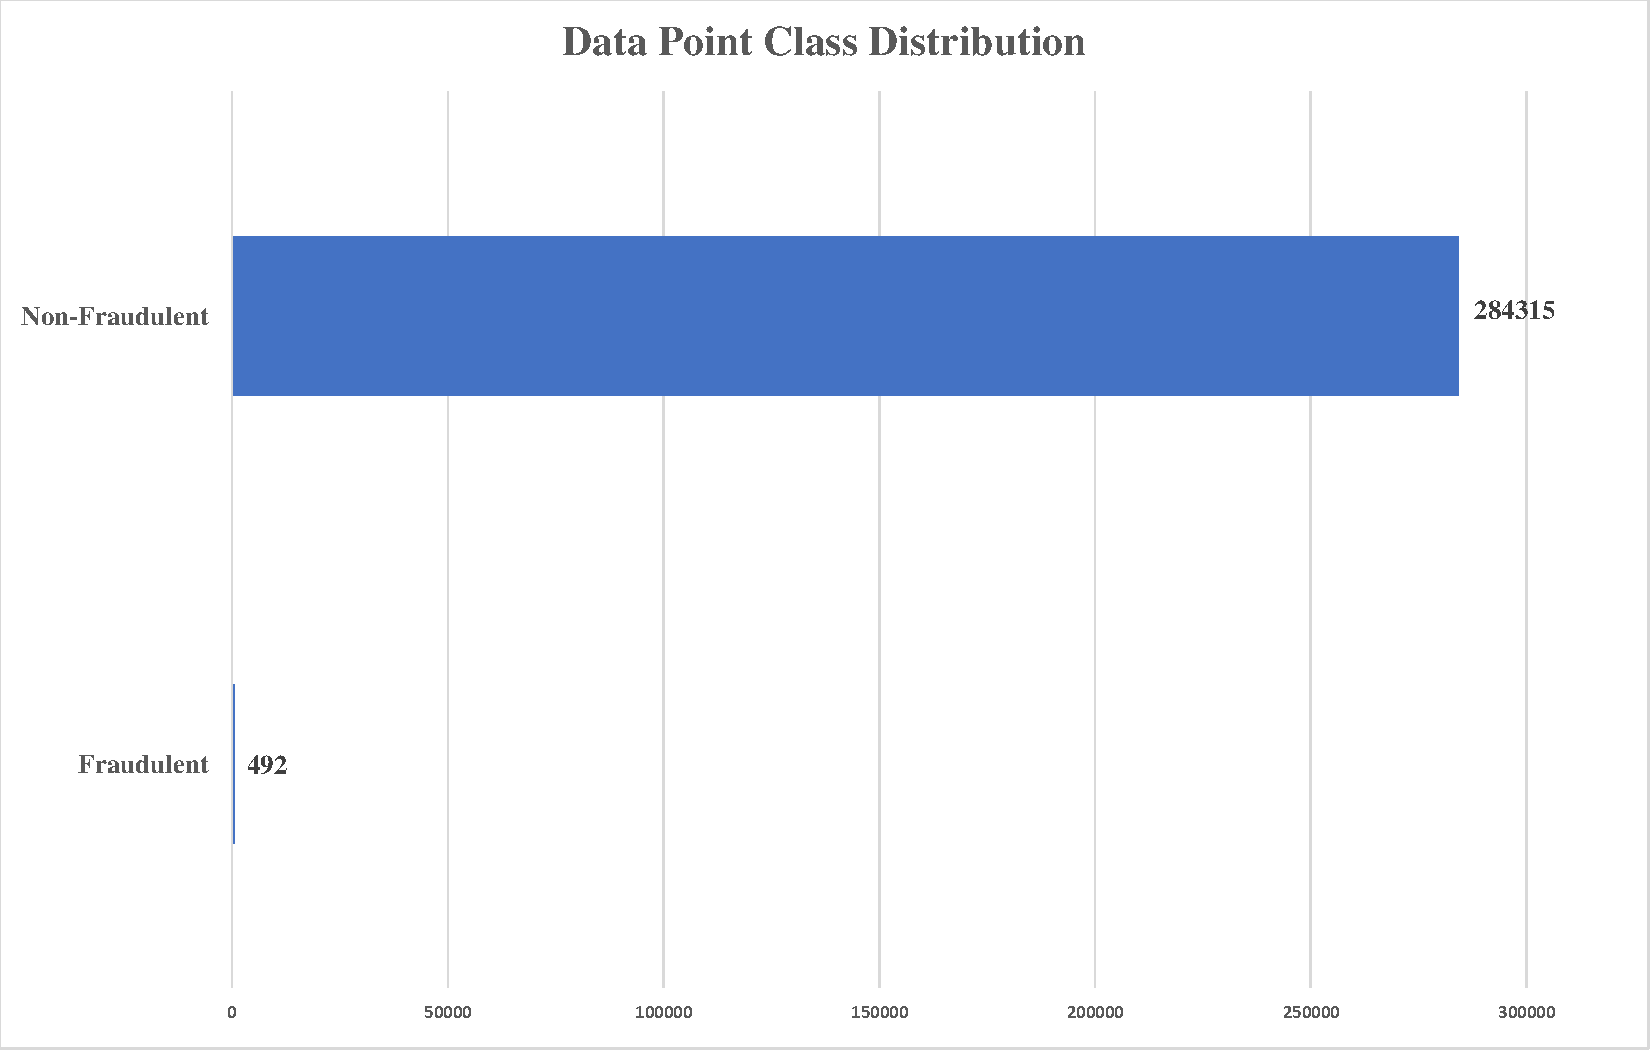
\includegraphics[width=100mm]{DataDistribution.pdf}
    \caption{Distribution between fraudulent and non-fraudulent data points.}
    \label{data-distribution}
  \end{center}
\end{figure}

 The fraudulent cases are also the most interesting result from the network, as simply identifying the 
 99.82800\% of non-fraudulent cases is trivial. The skewed distribution of data points is illustrated
 in Figure~\ref{data-distribution}.


\section{Methods}


\subsection{Deep Learning Framework}

 TensorFlow r1.8 was used to carry the back end of the neural network, providing definitions
 for layers, optimization functions, back propagation, and running of the network. The Pandas 
 package was used heavily for the data pre-processing and matrix manipulations.

\subsection{Data Pre-Processing}

 The dataset is provided in a .csv format, so the first pre-processing step is to read the data points 
 into the Pandas package. Once the data is read in, the “Class” property is changed into two properties,
 named “Fraud” and “NonFraud” for easier determination of the output of the network. The fraudulent 
 and non-fraudulent cases are then split into two lists for division of training and testing data. 75\% 
 of each case is used as training data, while the remaining  25\% is used for testing data. Both the 
 training and test data are further divided into various targeted lists for result processing later in the network.

\subsubsection{Augmentation of Fraudulent Cases}

 To overcome the skewed nature of the dataset, augmentation of the fraudulent cases is required. 
 Augmentation was accomplished by sampling the fraudulent cases in the training set 600 times, 
 to obtain a ratio between the training cases of around 50:50.


\subsection{Neural Network Architecture}

\begin{figure}
  \begin{center}
    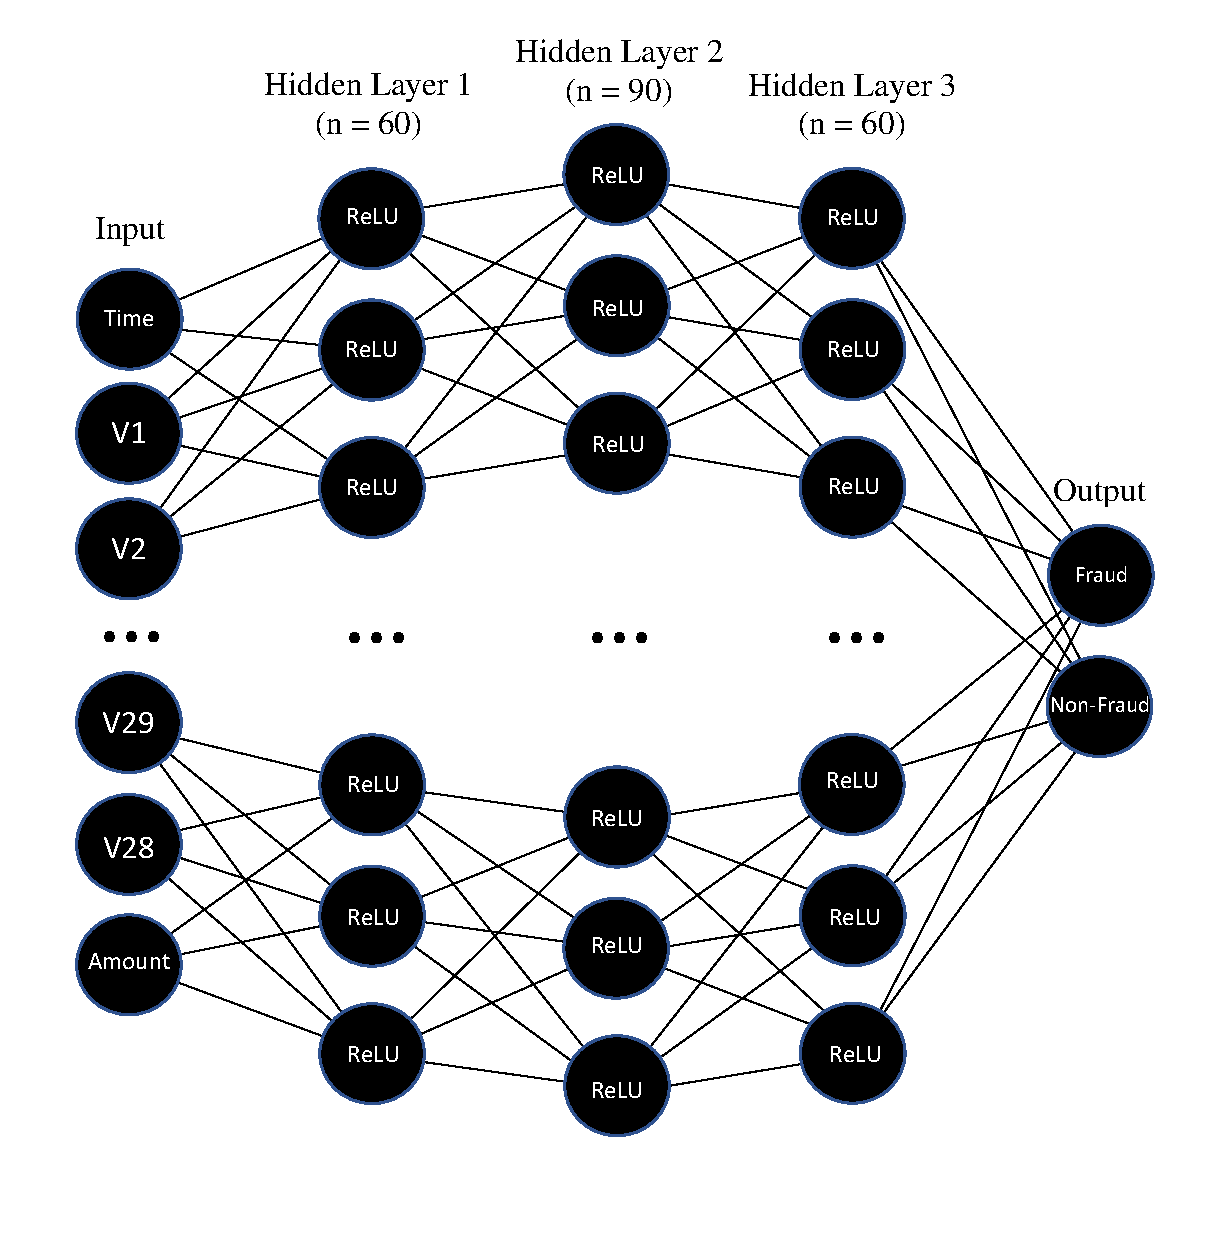
\includegraphics[width=100mm]{NeuralNetDiagramPDF.pdf}
    \caption{Diagram of neural network architecture (Bias nodes not included).}
    \label{network-architecture}
  \end{center}
\end{figure}

 \subsubsection{Layer Definitions}

 The neural network is defined by an input layer, three hidden layers, and an output layer, as can 
 be seen in Figure~\ref{network-architecture}. Each layer also includes a bias input. The input layer is the 
 width of each data point (30), with each layer doubling the width of the previous layer until the 
 output layer, which is of width 2. A fully connected network approach is also used.

\subsubsection{Weight and Bias Initializations}

 Each layer’s weights are initialized using a random generated number from a normal distribution 
 with a standard deviation of  0.1 and centered around zero. The bias weights are initialized in a 
 similar fashion.

\subsubsection{Activation Functions}

 Activation functions used between layers are rectified linear units (RELU), as well as a linear 
 activation function leading to the output layer. Each node also utilizes a dropout normalization
 strategy to avoid overfitting [2].

\subsubsection{Batch Strategies}

 There are two batch strategies used in the experiments. The first strategy is a simple, 
 even, and consistent division of the dataset throughout each epoch. The second strategy 
 is a random sequence selection from the dataset for each batch [3].

\subsubsection{Output Interpretation}

 The cost function used for interpretation of the network output is mean squared error (MSE) [4]. 
 The accuracy of the output is determined by selecting the index of the output node with higher 
 activation and comparing it to the index of the output node of the expected result.

\section{Experiments}

\subsection{Network Design}

\subsubsection{Initial Network Design}

 The network was initially designed using sigmoid activation functions with a cross entropy 
 cost function and a gradient descent optimizer. The preprocessing also did not augment 
 the fraudulent cases. As a result, the network would simply learn to identify the non-fraudulent 
 cases, reaching a 99.828\% overall accuracy, but completely missing the fraudulent cases, 
 which are the most interesting cases for the network to learn. Adjustments to hyperparameters 
 such as layer width, step size, and batch size were unable to overcome the bias for choosing all 
 cases as being non-fraudulent.

\subsubsection{Final Network Design}

 The network was able to identify fraudulent cases after a second pass of network and pre-processing 
 design. The network activations were changed to use ReLU activation functions to avoid the narrowing 
 of outputs. The cost function was switched to MSE to avoid the required clipping of outputs, as cross 
 entropy requires log functions which have a limited input range. The optimizer was also changed to 
 an Adam Optimizer. 

 Augmenting the fraudulent cases in the training data was the largest change for the final design 
 of the system. By sampling the training data 600 times, the number of cases were roughly even 
 between fraudulent and non-fraudulent. This allowed the test precision on fraudulent cases to 
 reach 75\% or greater, while the non-fraudulent precision also remained in the high  90\% range.

\subsection{Results}

 As a precursor to the results discussion, the first 50 epochs of the training process are being ignored,
 as these epochs experience extreme volatility, and throw off the analysis of results. This analysis is 
 also done over 350 epochs. Increasing the number of epochs may produce interesting results in the 
 late stage of learning. 

\subsubsection{Baseline Network Results}

 Using the above mentioned final network design, the network was able to produce a peak overall 
 test accuracy of 99.66995\%, with associated non-fraudulent and fraudulent detection rates of 
 99.70455\% and 79.6748\%, respectively. 

 Looking at the left hand side Figure~\ref{basline-random}, it can be seen that the network initially identifies all 
 cases as non-fraudulent, then moves towards a more 50/50 split between case predictions, and 
 finally learns the differentiation between cases, and both precision rates increase. Some of the
 noise in epoch ranges 150-250 is like attributed to the repeated test cases of the fraudulent type. 

 A precision of 99.70455\% in detecting non-fraudulent cases correctly may seem quite high,
 but a false positive rate of 0.29545\% is most likely unacceptable to a credit card company,
 as hundreds of thousands of transactions occur daily.


\subsubsection{Results Using Pseudo-Random Batches}

 Using pseudo-random batch selection, the network reached a top overall test accuracy of 99.76124\%,
 with this instance of the network also maintaining a 99.798816\% precision in marking non-fraudulent 
 cases, and a 78.04878\% precision in marking fraudulent cases. 

 In comparison to the baseline network results, as can be seen in Figure~\ref{basline-random},  
 using pseudo-random batch generation appears to give more consistent results throughout epochs.
 The pseudo-random batch approach can also improve the identification rate in the non-fraudulent cases.

\begin{figure}
  \begin{center}
    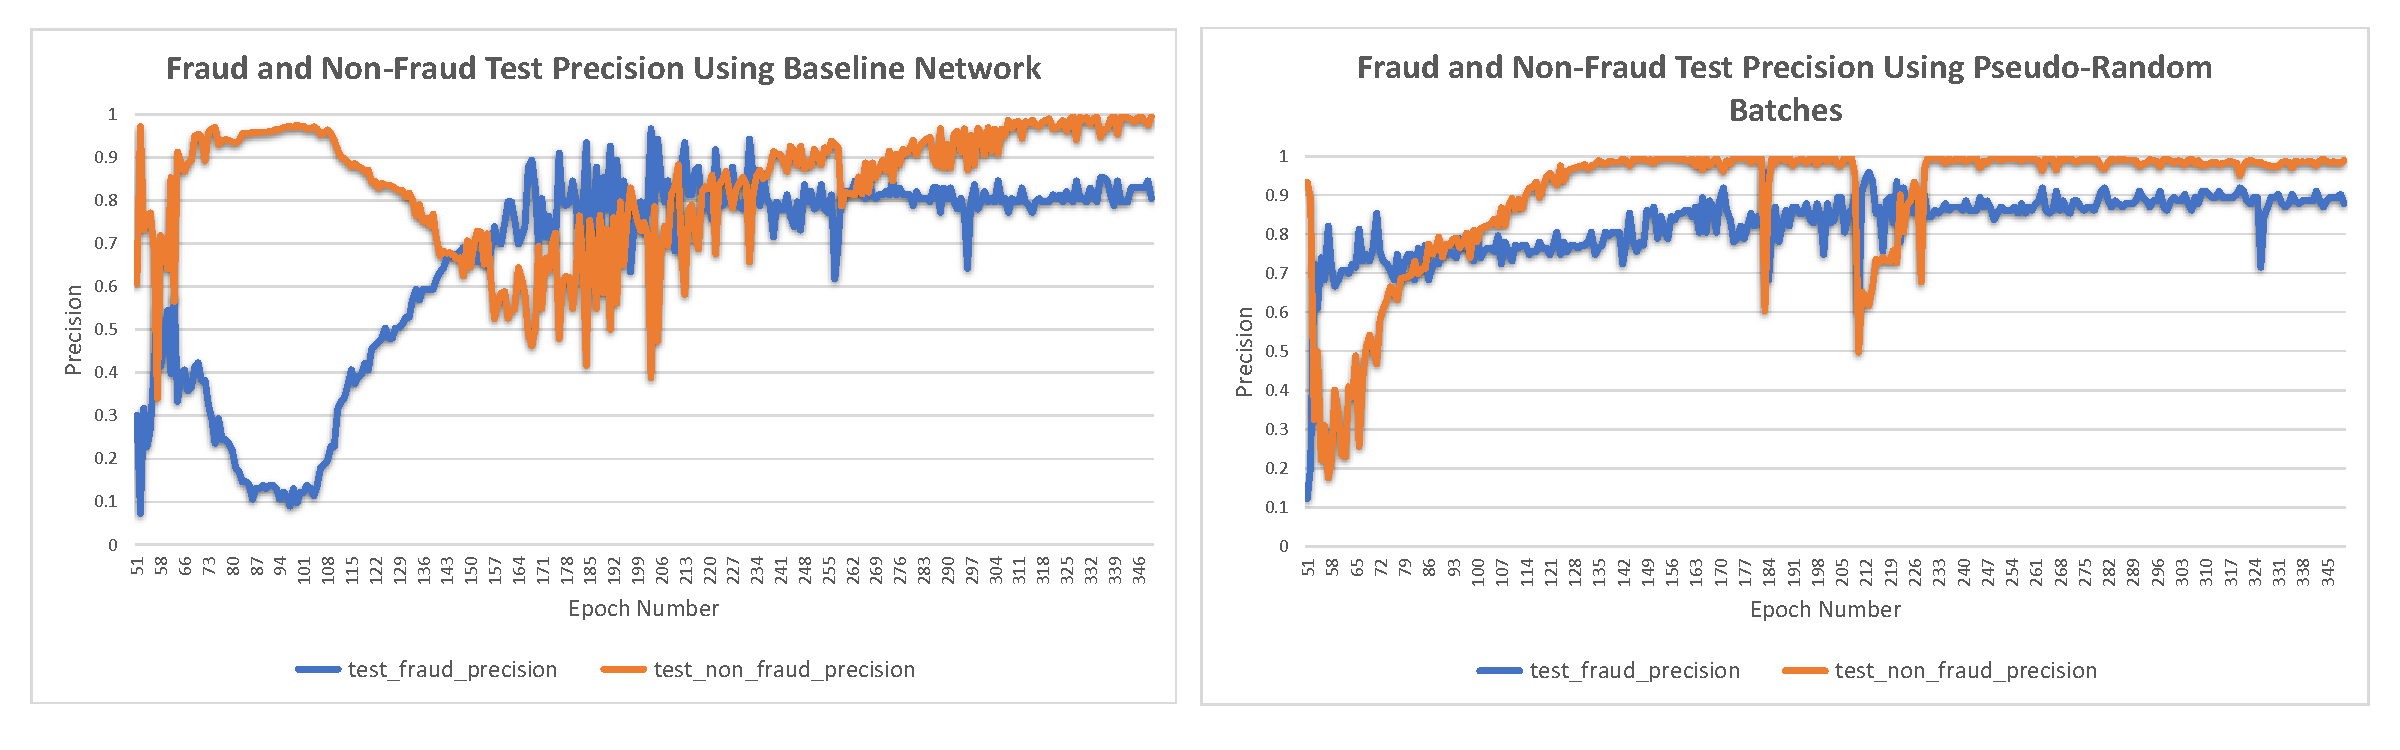
\includegraphics[width=135mm]{FraudNonFraudTestPrecision.pdf}
    \caption{Comparison of baseline batch and pseudo-random batch results.}
    \label{basline-random}
  \end{center}
\end{figure}

\subsubsection{Results Using a Modified Learning Rate}

 The baseline network uses a learning rate hyperparameter of 1e-5. To test the effect of
 manipulating the learning rate, the network was also run with rates of 1e-4 and 1e-6.

The results of these learning rate adjustments are noted in Figure~\ref{learning-rate}.
 It is obvious that the baseline learning rate of 1e-5 performed the best. A learning rate
 of 1e-4 was completely unable to differentiate between the cases, giving an output of
 fraudulent for almost all cases. This is likely due to overstepping a minimum of the cost
 function. Using a learning rate of 1e-6 produced sporadic results for the first 150 epochs,
 until it finally began differentiating the cases slowly. With a few hundred more epochs, the
 network may have reached an accuracy similar to the baseline.

\begin{figure}
  \begin{center}
    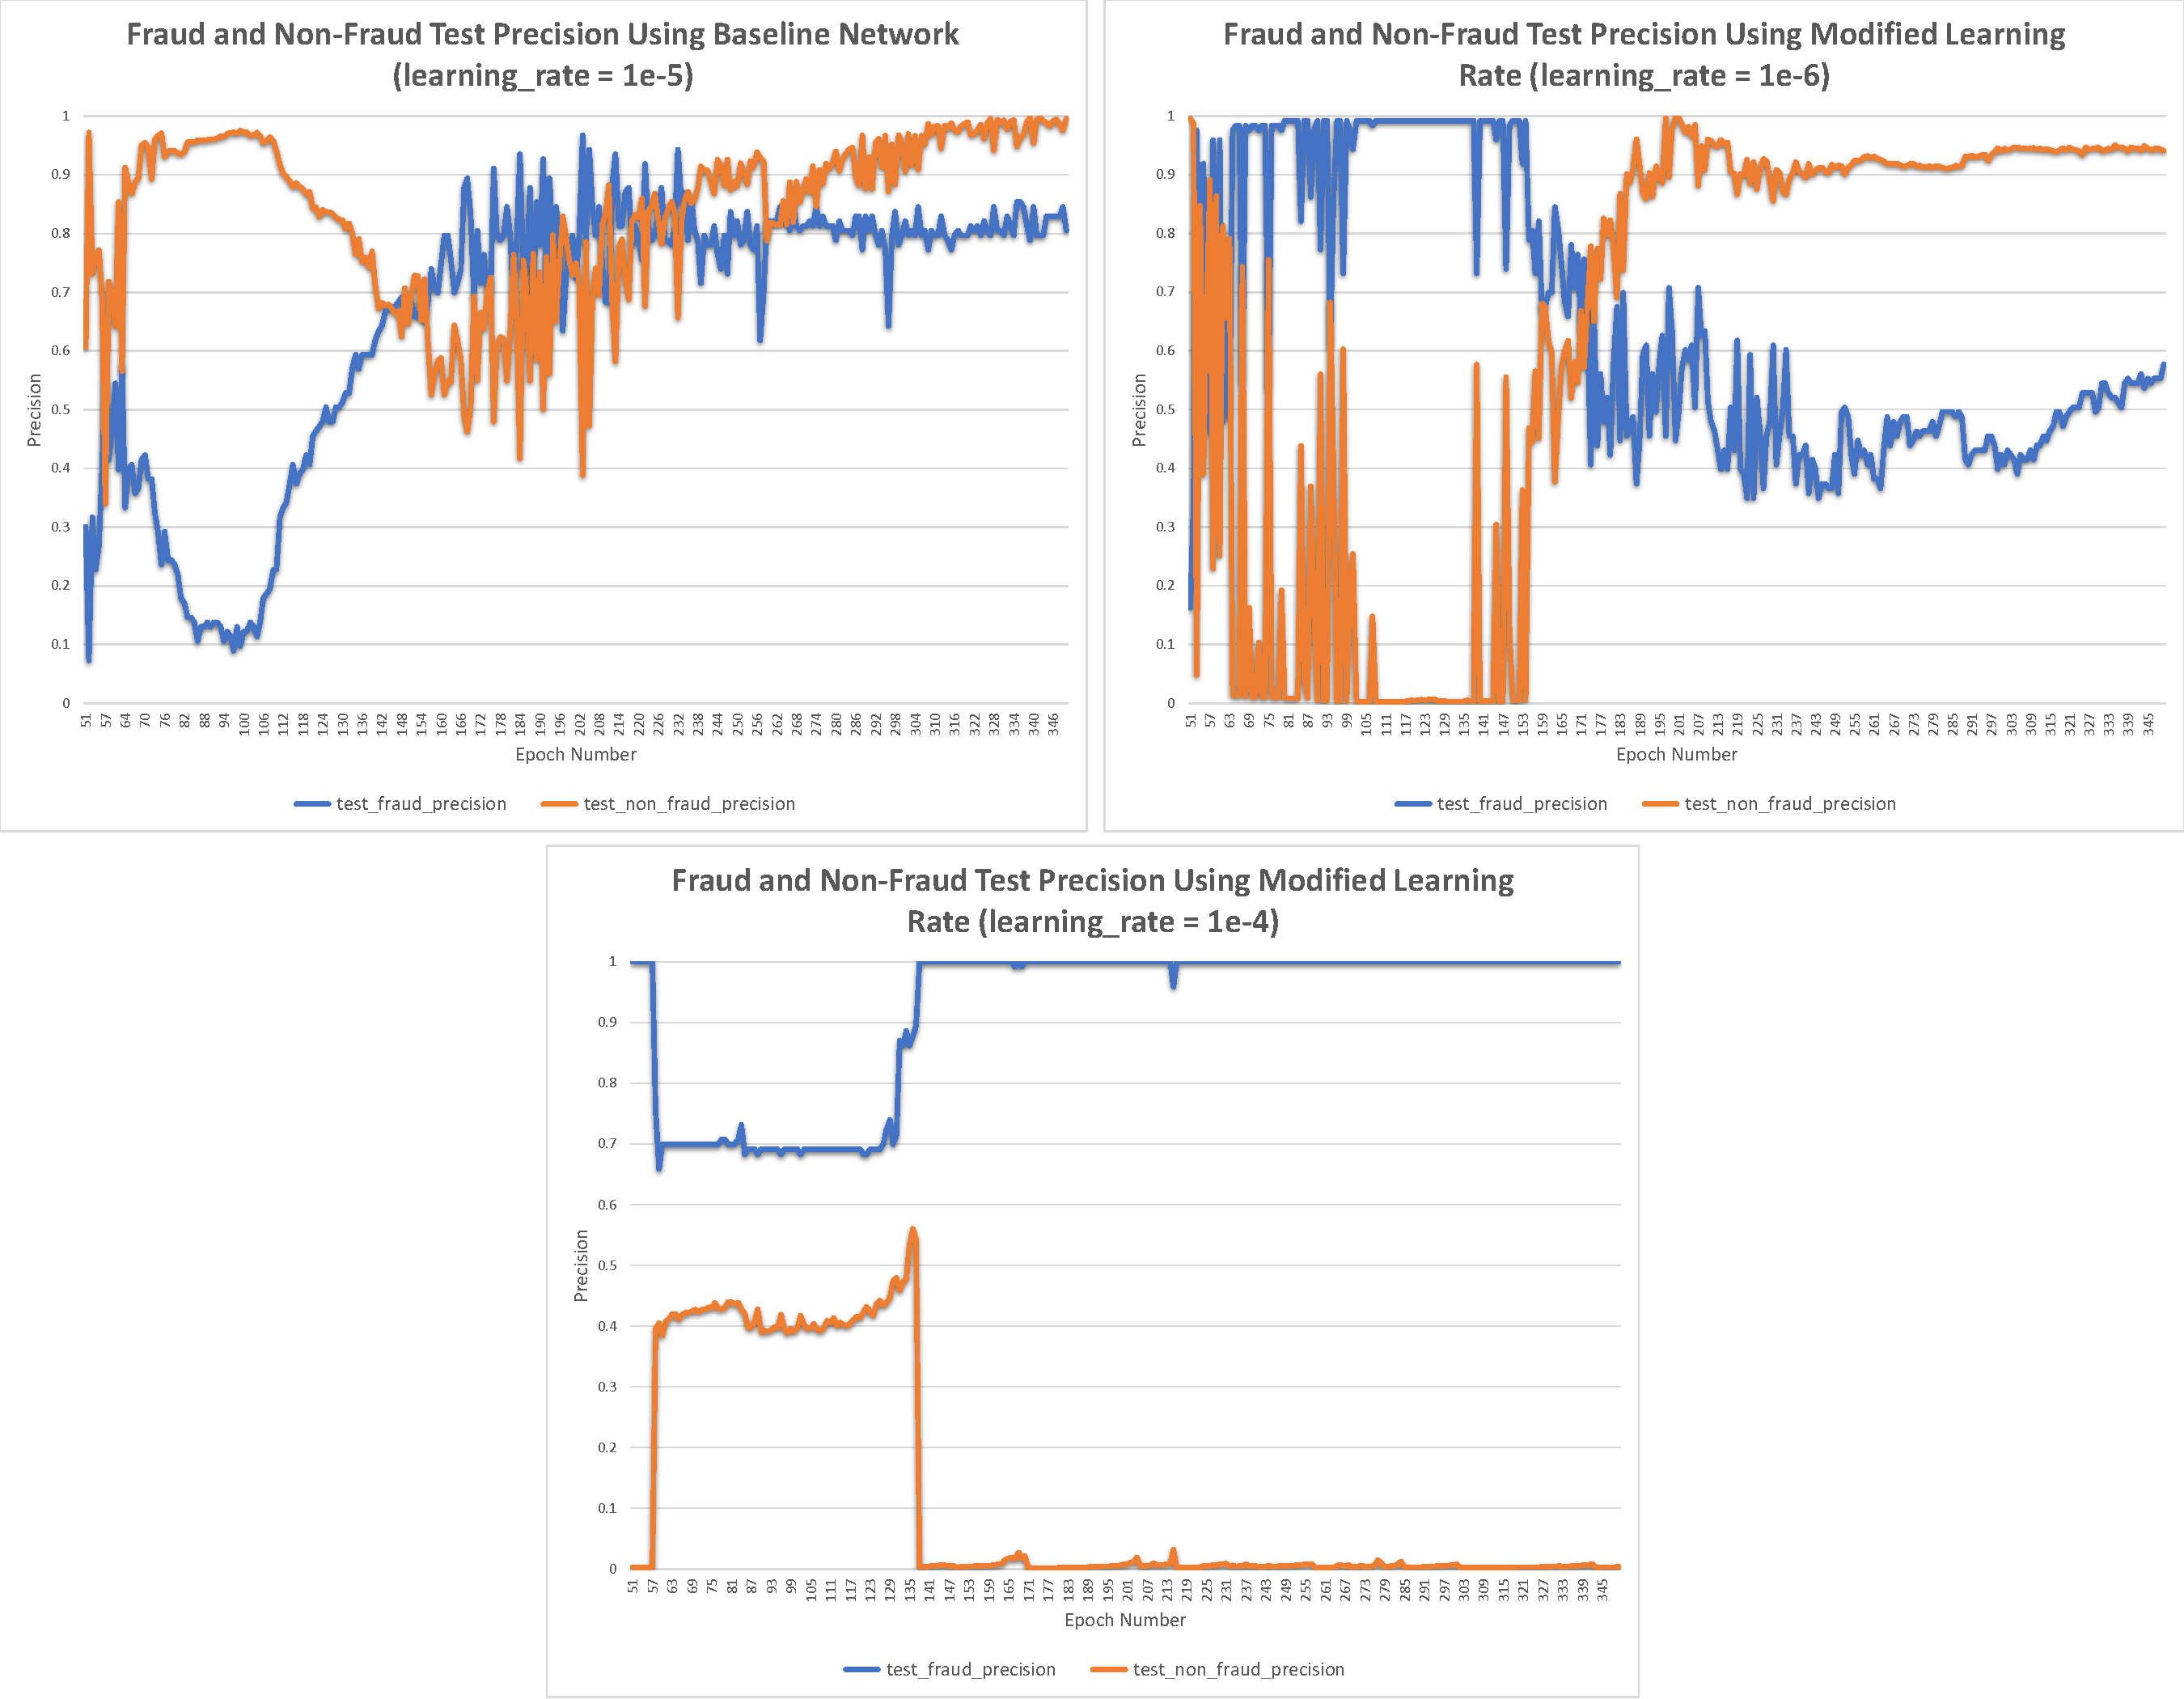
\includegraphics[width=135mm]{ModifiedLearningRate.pdf}
    \caption{Comparison of baseline and modified learning rate results.}
    \label{learning-rate}
  \end{center}
\end{figure}

\subsubsection{Results Using a Deeper Network}

A final modification to the baseline neural network that was experimented with was adjusting
 the depth of the network. A network using four hidden layers is compared to the baseline
 network of three hidden layers in Figure~\ref{deeper-network}. 

 The deeper network appears to make the differentiation between cases earlier than the
 shallow network, but in the end is unable to pick up on the small number of fraudulent cases.
 This could be due to a vanishing gradient issue due to the nature of a deep network using ReLU
 activation functions [5].

The deeper network ended up being able to producer a higher overall accuracy of 99.88483\%,
 but was only able to identify 39.8374\% of fraudulent cases at that accuracy level. The false
 positive rate of this network was only 0.011253\%, so it could still be a viable
 option for detecting fraud with higher confidence.

\begin{figure}
  \begin{center}
    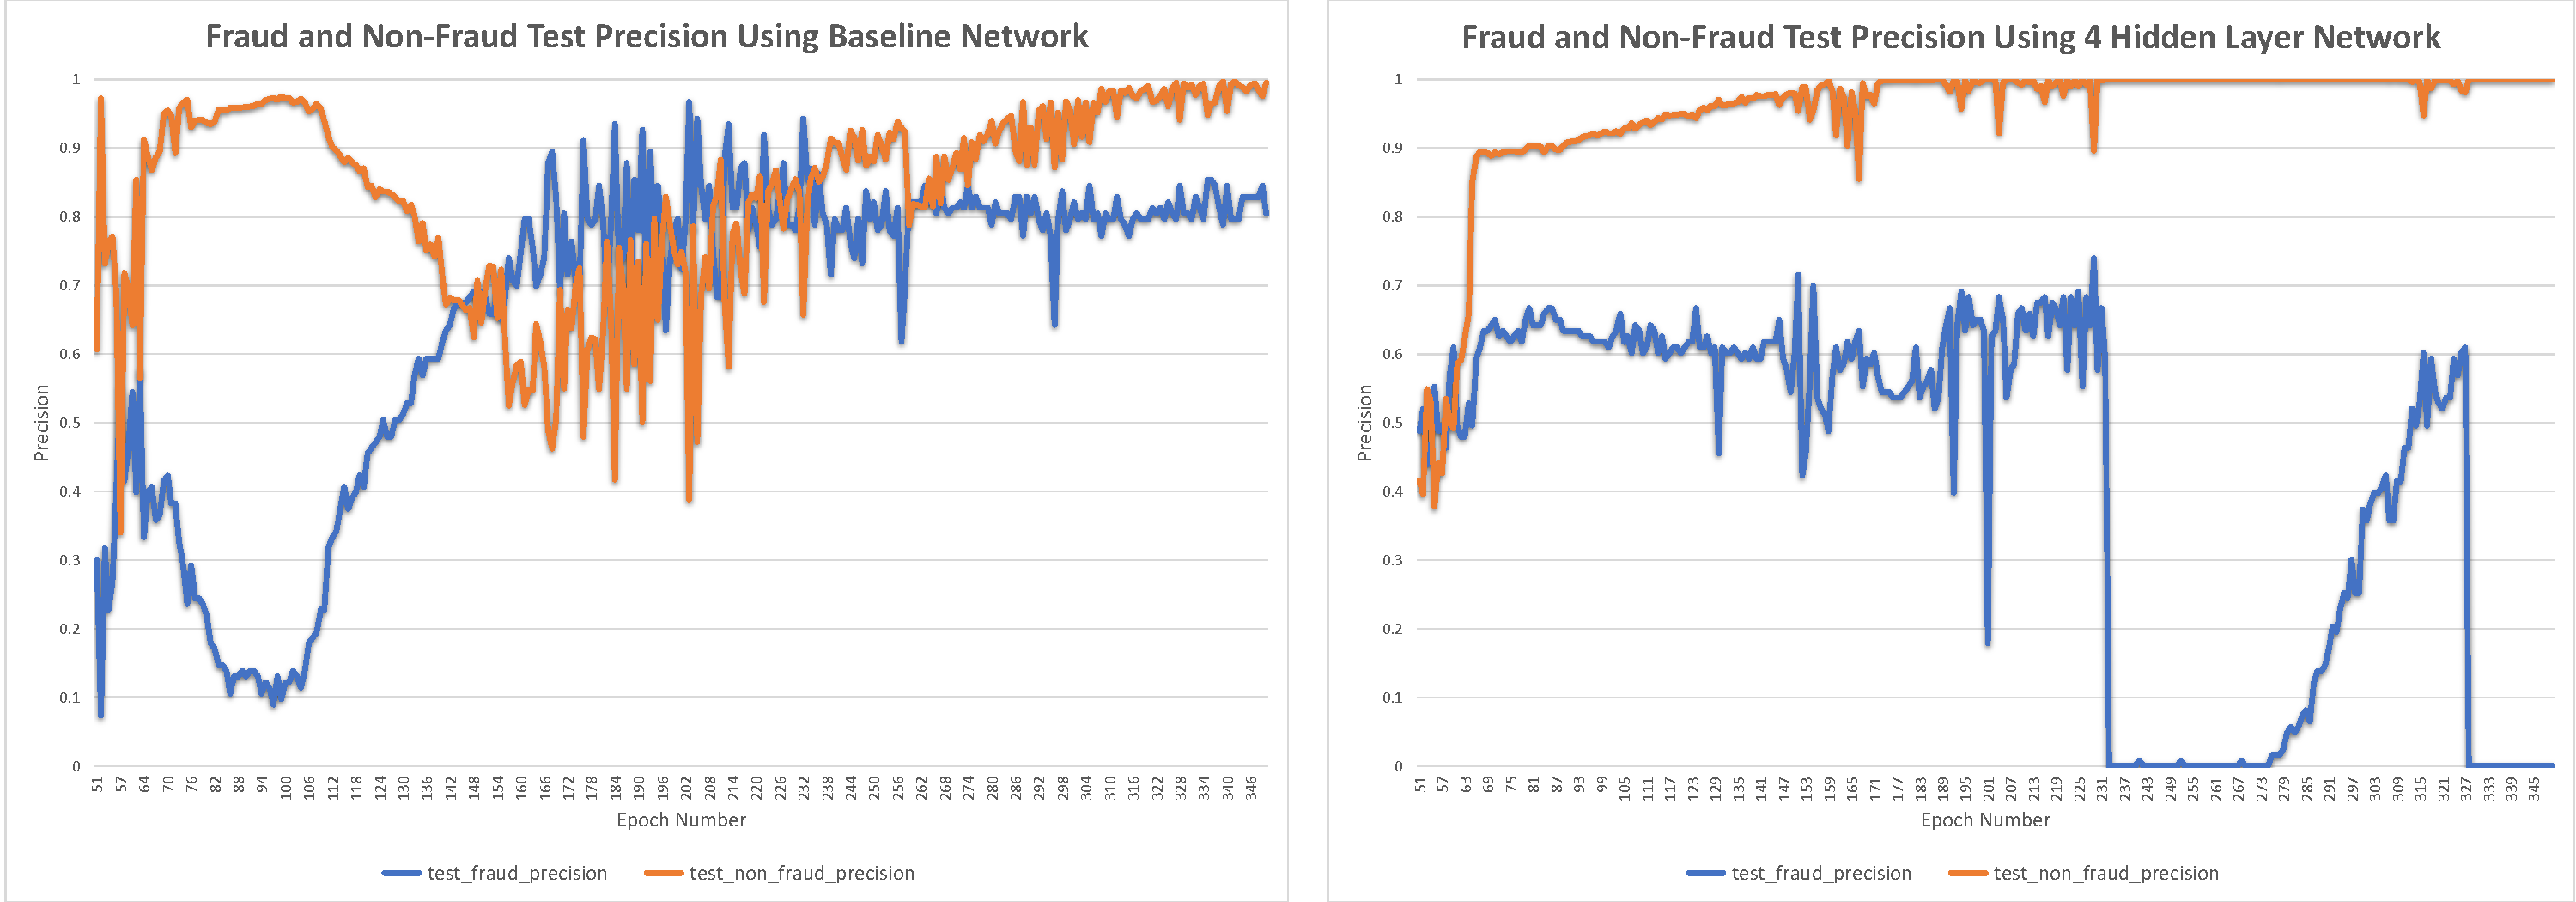
\includegraphics[width=135mm]{DeeperNetwork.pdf}
    \caption{Comparison of baseline and deeper network results.}
    \label{deeper-network}
  \end{center}
\end{figure}

\subsection{Summary of Results}

 To summarize the results of modifying the baseline network, using a pseudo-random batch
 generation strategy can produce better, more consistent overall results. Also using a higher
 or lower learning rate will likely not improve the performance of this network. Finally, using a
 deeper network may reduce the rate of false positives, but also fails to identify a much
 larger proportion of fraudulent cases.

\subsection{Sources of Error}

Potential errors in the results may be attributed to a few different causes. One
 would be the random initialization of the network, as some initializations may
 be more optimal than others when learning the differentiation of the cases. Each
 sample of learning was taken from a single random initialization of the network.
 Averaging multiple initialization results could give a better representation of the
 network’s typical results. Another source of issues could come from the limited
 range of epochs run through the network. Running the network for 350 epochs
 produces a relatively good representation of what the network is capable of
 learning. Using more epochs could produce slightly different results.

\subsection{Further Work}

This experiment could be furthered if there was a dataset found with more 
data points available for fraudulent transactions. The hyperparameter 
optimization could also be further explored.

\section{Conclusion}

As can be seen, a deep neural network is capable of learning to differentiate between
 fraudulent and non-fraudulent credit card transactions. With accuracy rates over 99\%,
 this approach is viable to the credit card industry with a few modifications to weed out
 false positives on non-fraudulent cases.

\section*{References}

\small

[1] “Consumer Sentinel Network Data Book 2017: Report Categories.” Federal Trade Commission, 
Federal Trade Commission, 6 Mar. 2018, www.ftc.gov/policy/reports/policy-reports/commission-staff-reports/consumer-sentinel-network-data-book-2017/report-categories.

[2] Srivastava, Nitish, et al. “Dropout: A Simple Way to Prevent Neural Networks from Overfitting.” Journal of Machine Learning Research 15, June 2014

[3] Loffe, Sergey, and Christian Szegedy. “Batch Normalization: Accelerating Deep Network Training by Reducing Internal Covariate Shift.” Cornell University Library, 2 Mar. 2015, arxiv.org/abs/1502.03167.

[4] Wang, Zhou, and Alan C. Bovik. “Mean Squared Error: Love It or Leave It? A New Look at Signal Fidelity Measures.” IEEE Xplore, IEEE, 13 Feb. 2009, ieeexplore.ieee.org/abstract/document/4775883/?part=1.

[5] Huang, Gao, et al. “Deep Networks with Stochastic Depth.” SpringerLink, Springer, Cham, 8 Oct. 2016, link.springer.com/chapter/10.1007/978-3-319-46493-0\_39.


\end{document}
